\begin{figure}[ht]
\centering
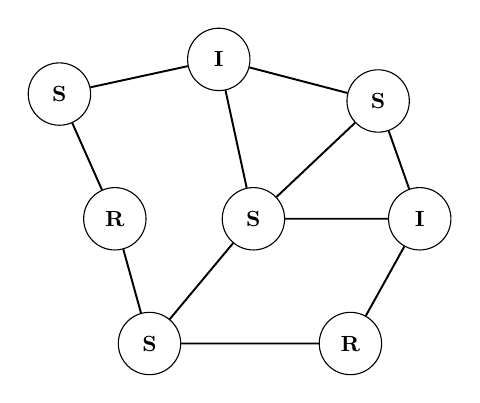
\begin{tikzpicture}[scale=0.88, every node/.style={transform shape},
 contato/.style={line width=.7pt},
 pessoa/.style={circle,draw=black,minimum size=9mm,inner sep=0pt,font=\small\bfseries,fill=white}]
\node[pessoa] (a) at (0,1.8) {S};
\node[pessoa] (b) at (2.3,2.3) {I};
\node[pessoa] (c) at (4.6,1.7) {S};
\node[pessoa] (d) at (0.8,0) {R};
\node[pessoa] (e) at (2.8,0) {S};
\node[pessoa] (f) at (5.2,0) {I};
\node[pessoa] (g) at (1.3,-1.8) {S};
\node[pessoa] (h) at (4.2,-1.8) {R};
\draw[contato] (a)--(b)--(c)--(f)--(h)--(g)--(d)--(a);
\draw[contato] (b)--(e)--(g) (c)--(e) (e)--(f);
\end{tikzpicture}
\caption{Exemplo ilustrativo de grafo de contatos com estados SIR (não representa dados reais).}
\label{fig:rede}
\end{figure}
